\documentclass[12pt,a4paper,twoside]{article}
\usepackage{labor}
\begin{document}

%fill for cover and header creation
\newcommand\laboratorynumber{2}
\title{Oszillograph}
\newcommand\supervisor{Ditlbacher, Harald}
\newcommand\groupnumber{42}

\newcommand\participantonelastname{Eisner}
\newcommand\participantonefirstname{Nico}
\newcommand\participantoneid{12214121}
\newcommand\participanttwolastname{Waldl}
\newcommand\participanttwofirstname{Philip}
\newcommand\participanttwoid{12214120}
\author{\participantonelastname \ \& \participanttwolastname}

\newcommand\degreeid{UB 033 678}
\newcommand\semester{23WS}
\date{20.10.2023}

%select correct course title
%\newcommand\coursetitle{Einführung in die \\ physikalischen Messmethoden}
%\newcommand\coursetitle{Laborübungen 1: \\ Mechanik und Wärme}
\newcommand\coursetitle{Laborübungen 2: \\ Elektrizität, Magnetismus, Optik}
%\newcommand\coursetitle{Fortgeschrittenen Praktikum 1: \\ Technische Physik}
%\newcommand\coursetitle{Fortgeschrittenen Praktikum 2: \\ Allgemeine Physik}

%\begin{titlepage}
   \begin{center}
       \begin{figure}[H]
            \begin{minipage}[h]{30mm}
                \centerline{
\includegraphics[height=15mm]{cover_nudes/tugraz.png}}
            \end{minipage}
            \hfill
            \begin{minipage}[h]{30mm}
                \centerline{
\includegraphics[height=15mm]{cover_nudes/nawi_graz.png}}
            \end{minipage}
            \hfill
            \begin{minipage}[h]{30mm}
                \centerline{
\includegraphics[height=15mm]{cover_nudes/uni-graz.png}}
            \end{minipage}
        \end{figure}
        
        \large{\emph{Institut für Experimentalphysik der Technischen Universität Graz \\
        \& Institut für Physik der Universität Graz}} \\
        \vspace{5mm}
        
        {\Huge \textbf{\coursetitle}}
        \vspace{5mm}
        
        {\huge \laboratorynumber: \thetitle}
    \end{center}
    
    \vfill
    
    \begin{table}[H]
        \LARGE
        \centering
        \begin{tabular}{r l}
            Betreuer:       & \supervisor \\
            Gruppennummer:  & \groupnumber \\
            \\
            Name:           & \participantonelastname, \participantonefirstname \\
            Matrikelnummer: & \participantoneid \\
            Name:           & \participanttwolastname, \participanttwofirstname \\
            Matrikelnummer: & \participanttwoid \\
            \\
            Kennzahl:       & \degreeid \\
            Datum:          & \semester \ | \thedate
        \end{tabular}
    \end{table}
    \vspace{4cm}
\end{titlepage}
\clearpage
\setcounter{page}{1}

%\maketitle %short title alternative

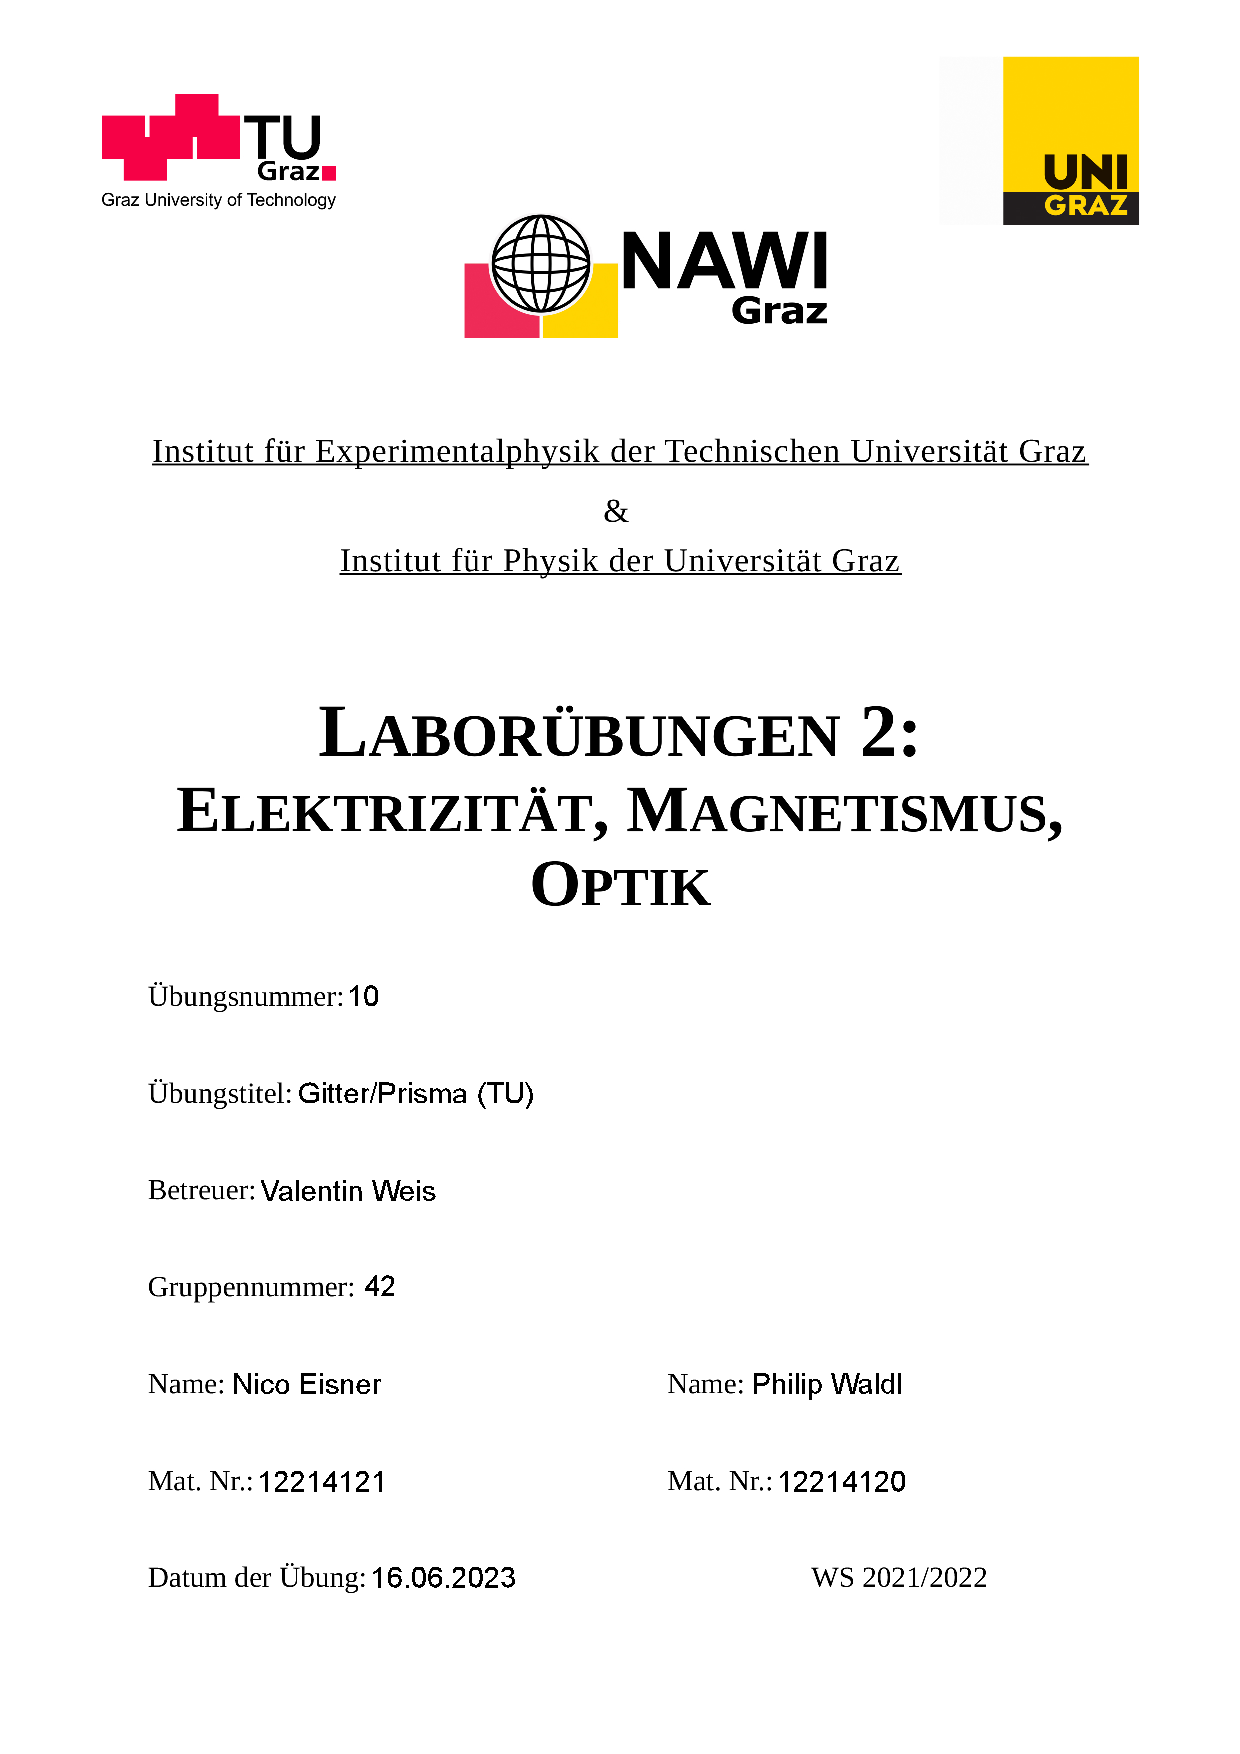
\includepdf[pages={1}]{../Deckblätter/Deckblatt_Gitter.pdf}

\tableofcontents
\newpage

\section{Aufgabenstellung} %jo beschreibn wos gmocht host ------------------------------

Der Versuch Oszillograph geht, wie der Name bereits vermuten lässt, auf die Funktion des Oszilloskopes ein, was in erster Linie die grafische Darstellung elektrischer Spannungen über einen bestimmten Zeitraum beinhaltet.
Mit drei verschiedenen elektrischen Schaltungen soll dies ausprobiert und in diesem Protokoll veranschaulicht werden. 
Die tatächliche Aufgabenstellung sieht hierfür wie folgt aus:

\begin{itemize}
    \item Serienschaltung (Trafo, Kondensator, Widerstand)
    \begin{itemize}
        \item Ermittlung des Phasenversatzes $\phi$
        \item Ermittlung von der Zerfallskonstante $\tau$
    \end{itemize}
    \item Serienschwingkreis (Trafo, Kondensator, Widerstand, Potentiometer)
    \begin{itemize}
        \item Zeichnen der von Kriechfall, Schwingfall, Aperiodischer Grenzfall des Serienschwingkreises
        \item Induktion der Spulte mit und ohne Eisenkern $L_{mitEisenkern}$ / $L_{ohneEisenkern}$
    \end{itemize}
    \item Frequenzbestimmung (Piezo)
    \begin{itemize}
        \item Eigenfrequenz des Stuhles $f_{Stuhl}$
        \item Eigenfrequenz des Piezos $f_{Piezo}$
    \end{itemize}
\end{itemize}

\noindent
Alle Informationen und Methodiken wurden uns von der Technischen Universität bereitgestellt \cite{teachcenter1}. 



\section{Voraussetzungen \& Grundlagen} %Grundlagen erklären, Formeln mit erklärung

Wie bereits in der Aufgabenstellung erwähnt werden Oszilloskope hauptsächlich zur grafischen Darstellung elektrischer Spannungen eingesetzt.  
Das Hauptbestandsteil des Gerätes ist eine Braun'sche Röhre und sieht im groben Aufbau wie folgt aus:

\begin{figure}[H]
    \centering
    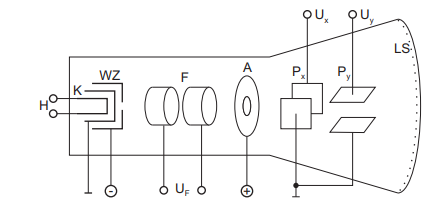
\includegraphics[width=0.5\linewidth]{nudes/OszilloskopAufbau.png}
    \caption{Grundlegender Aufbau eines Oszilloskop/Braun'sche Röhre \cite{teachcenter1}}
    \label{fig:Aufbau Oszilloskop}
\end{figure}

\noindent
Die beheizte Kathode K beschleunigt Elektronen gegen eine Anode A. Diese besitzt eine Öffnung, durch die die Elektronen hindurchfliegen und mit Hilfe der Ablenkplatten $P_{x}$ (horizontal) und $P_{y}$ (vertikal) an die richtige Position des Leuchtschirms LS gelenkt werden. 
Ein Oszilloskop besitzt außerdem einen Triggerungsmechanismus. Dieser sorgt dafür, dass das Signal beim erreichen des Bildschirmendes kurz pausiert wird, damit dieses wieder zum Anfang springen kann. \newline

\noindent
Zur erfolgreichen Durchführung des Versuches ist auch der Schwingkreis von Bedeutung. Dies ist im Prinzip eine einfache Schaltung, bestehend aus Kapazität, Induktivität und Widerstand.
Mittels Gleichung

    \begin{equation}
        \label{eq:SchwingkreisGleichungFälle}
        \centerline{$\lambda^2 + \lambda \frac{R}{L} + \frac{1}{LC} = 0 $}
    \end{equation}

\noindent
können hier drei verschiedene Fälle unterschieden werden:

\begin{itemize}
    \item $R^2C - 4L$ > 0: Kriechfall
    \item $R^2C - 4L$ = 0: Aperiodischer Grenzfall
    \item $R^2C - 4L$ < 0: Schwingfall
\end{itemize}

\section{Versuchsanordnung} %mit skizze kurz beschreiben ------------------------------

Als Grundstein des gesamten Experimentes steht natürlich das Oszilloskop, abgebildet in nachstehender Grafik.

\begin{figure}[H]
    \centering
    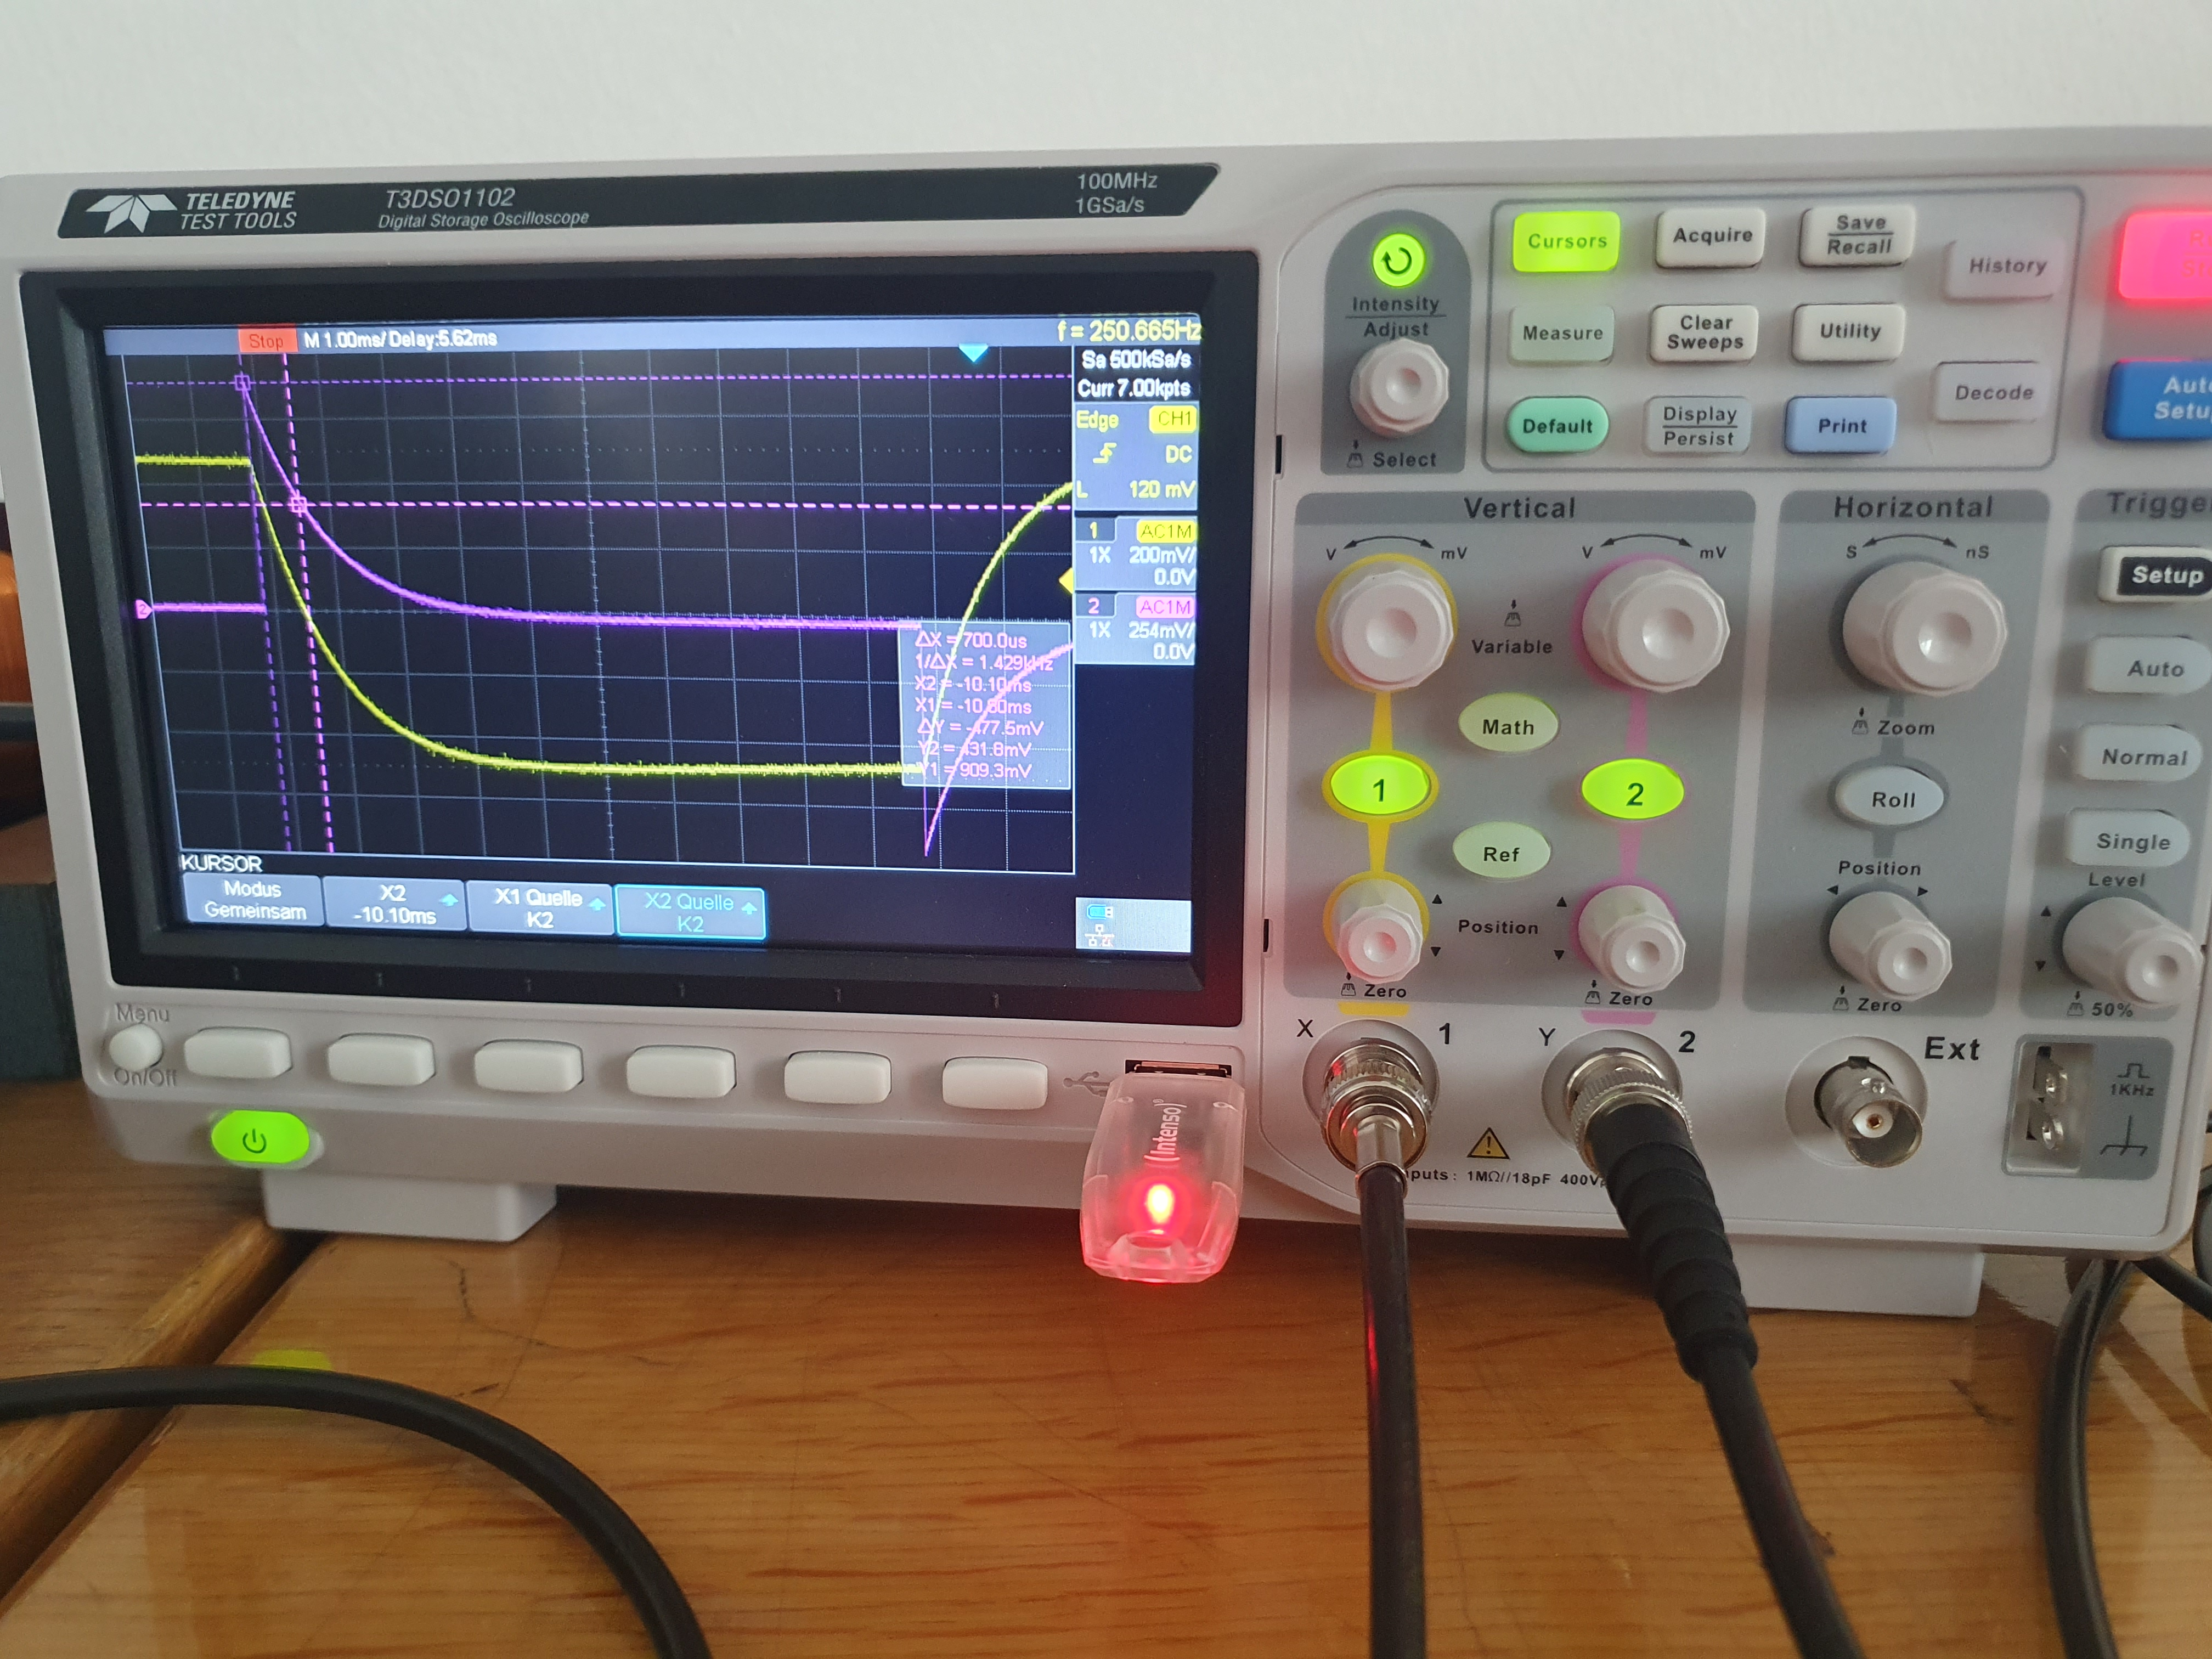
\includegraphics[width=0.6\linewidth, angle=0]{nudes/Osziloskop.jpg}
    \caption{Oszilloskop}
    \label{fig:Oszilloskop}
\end{figure}

\noindent
Auch Trafo und Frequenzgenerator, zu sehen in folgenden Abbildungen, sind weitere, wichtige Elemente des Versuches. 

\begin{figure}[H]
    \centering
    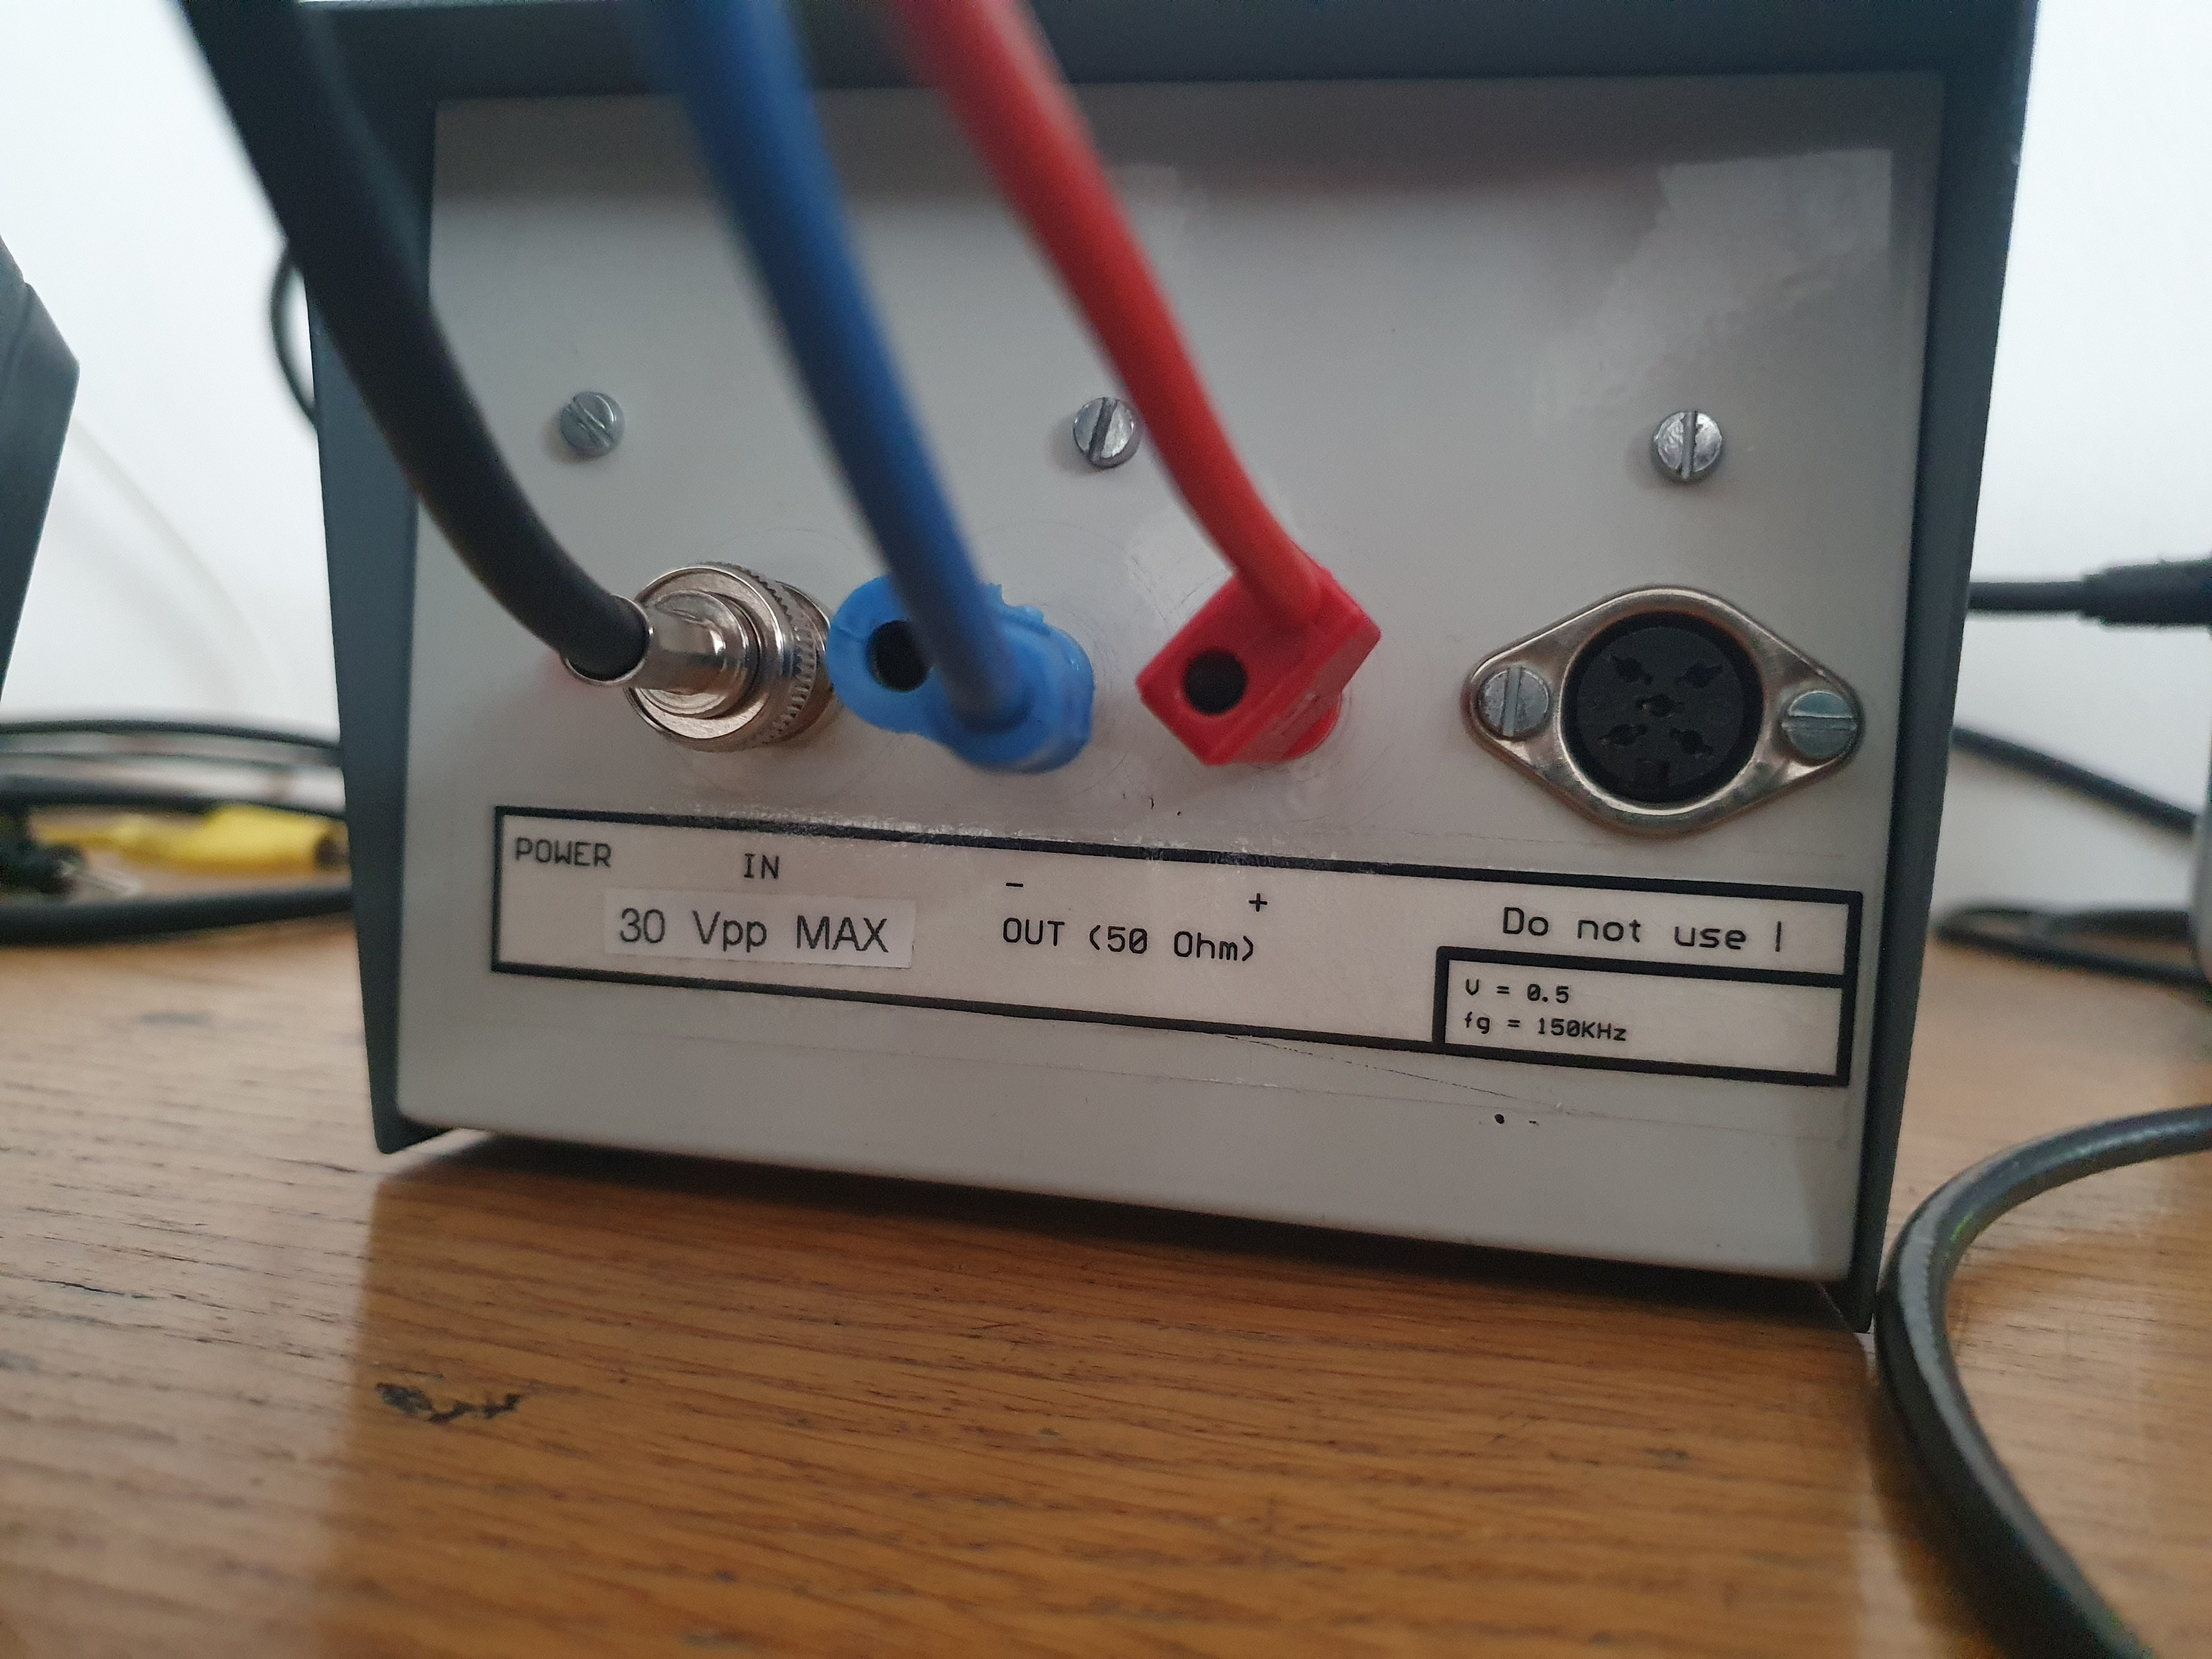
\includegraphics[width=0.6\linewidth, angle=0]{nudes/Trafo.jpg}
    \caption{Trafo}
    \label{fig:Trafo}
\end{figure}

\begin{figure}[H]
    \centering
    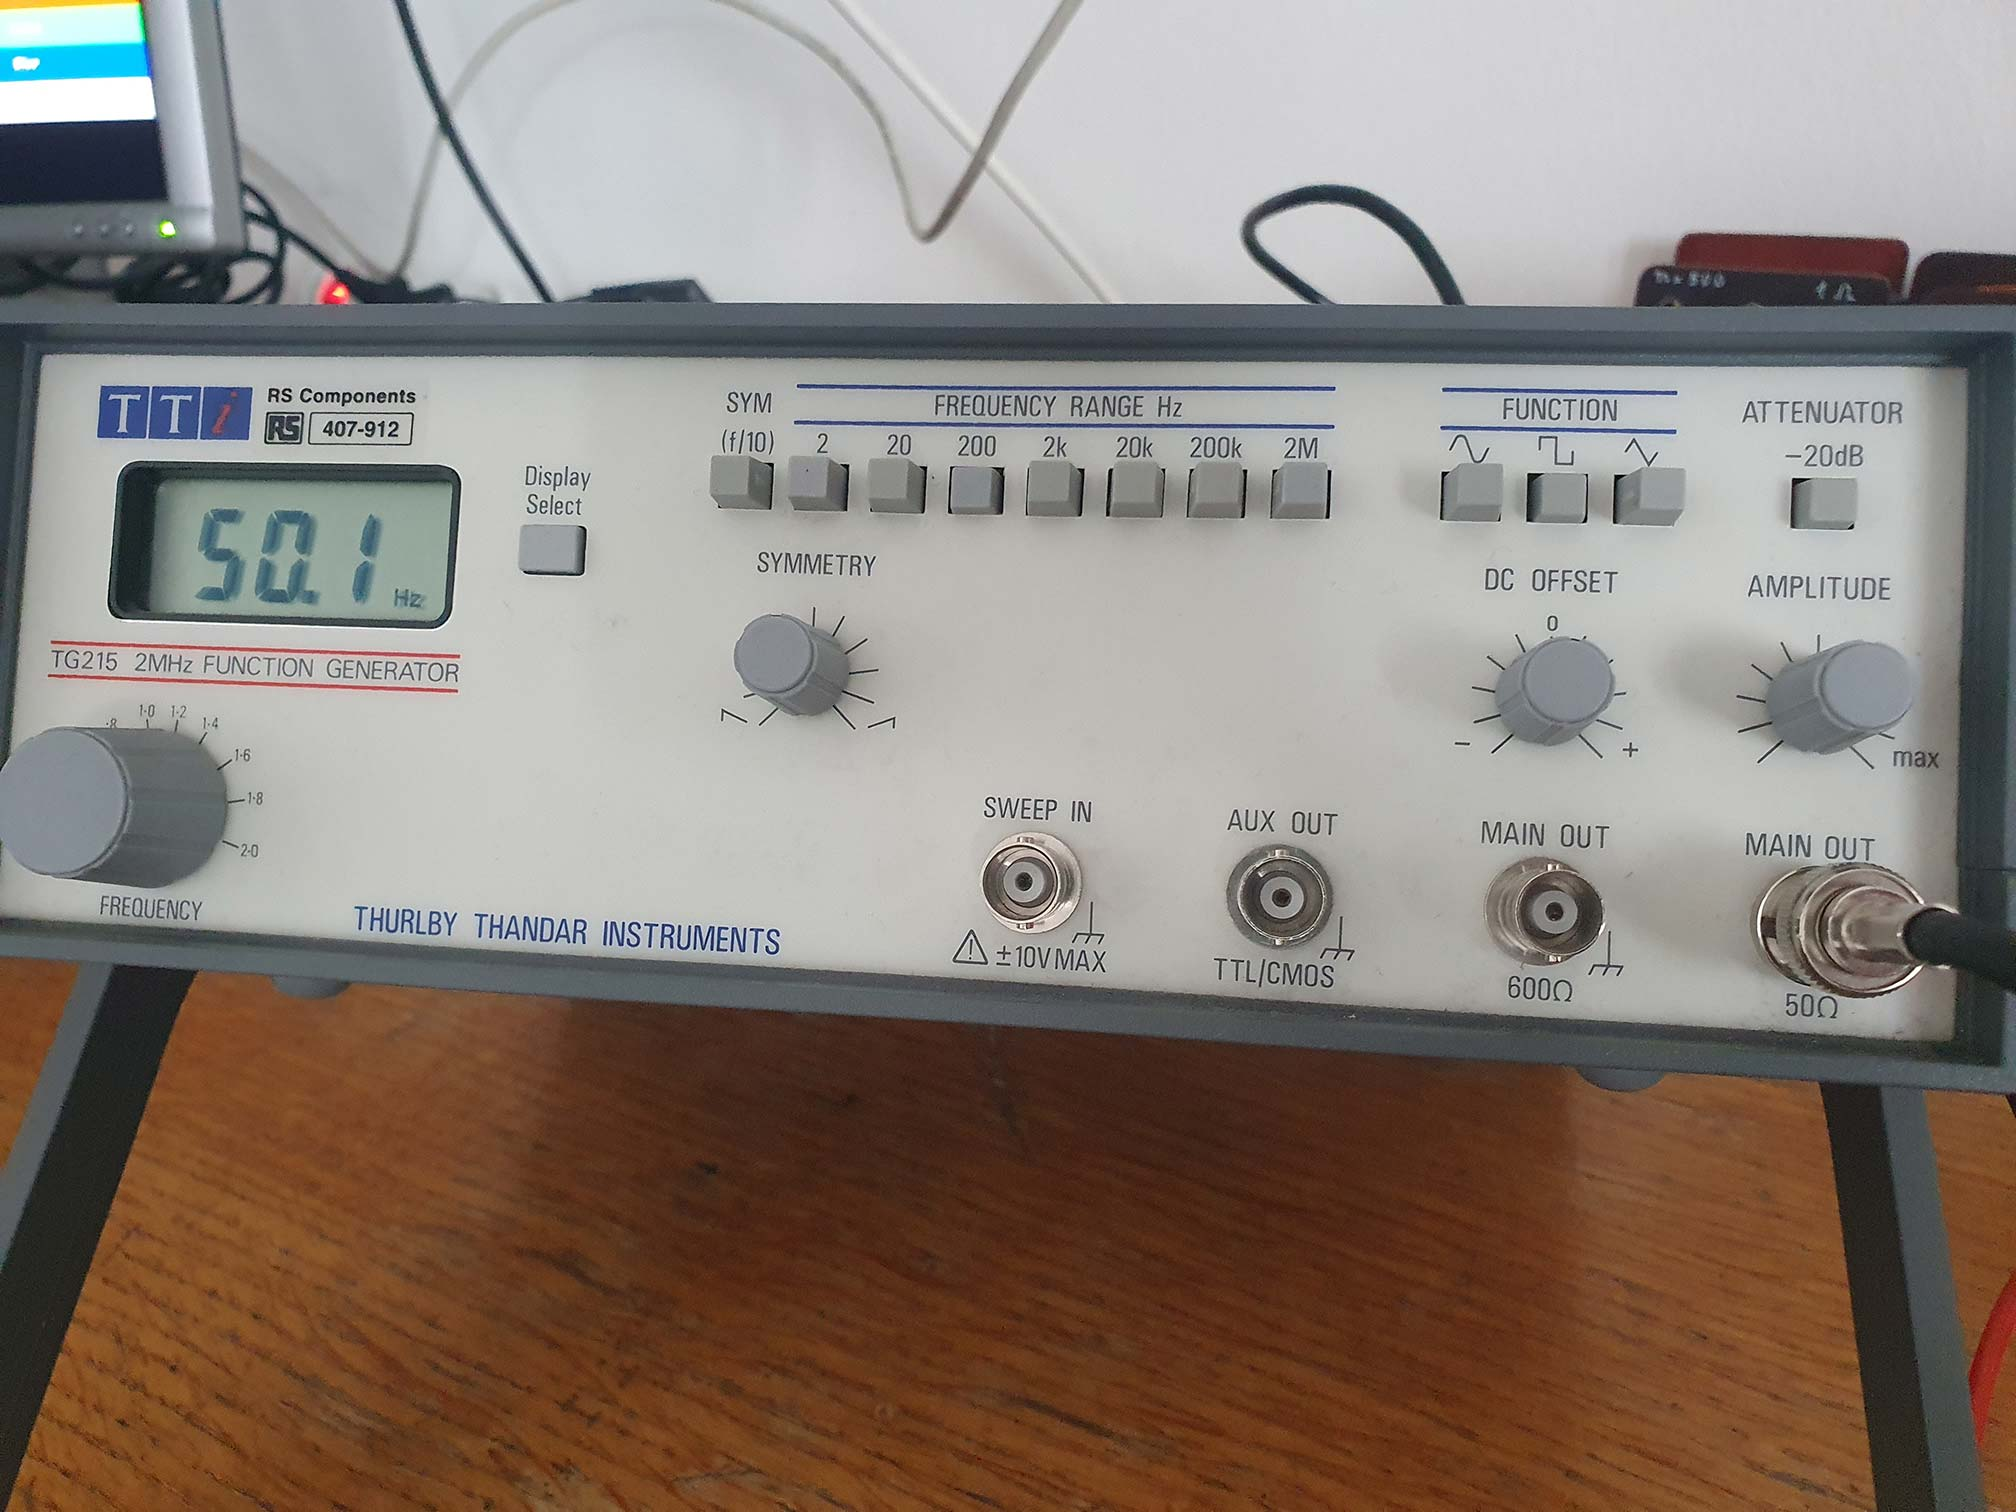
\includegraphics[width=0.6\linewidth, angle=0]{nudes/Frequenzgenerator.jpg}
    \caption{Frequenzgenerator}
    \label{fig:Frequenzgenerator}
\end{figure}

\noindent
Weiters kamen dann noch einige kleinere Utensilien zum Einsatz:

\begin{figure}[H]
    \centering
    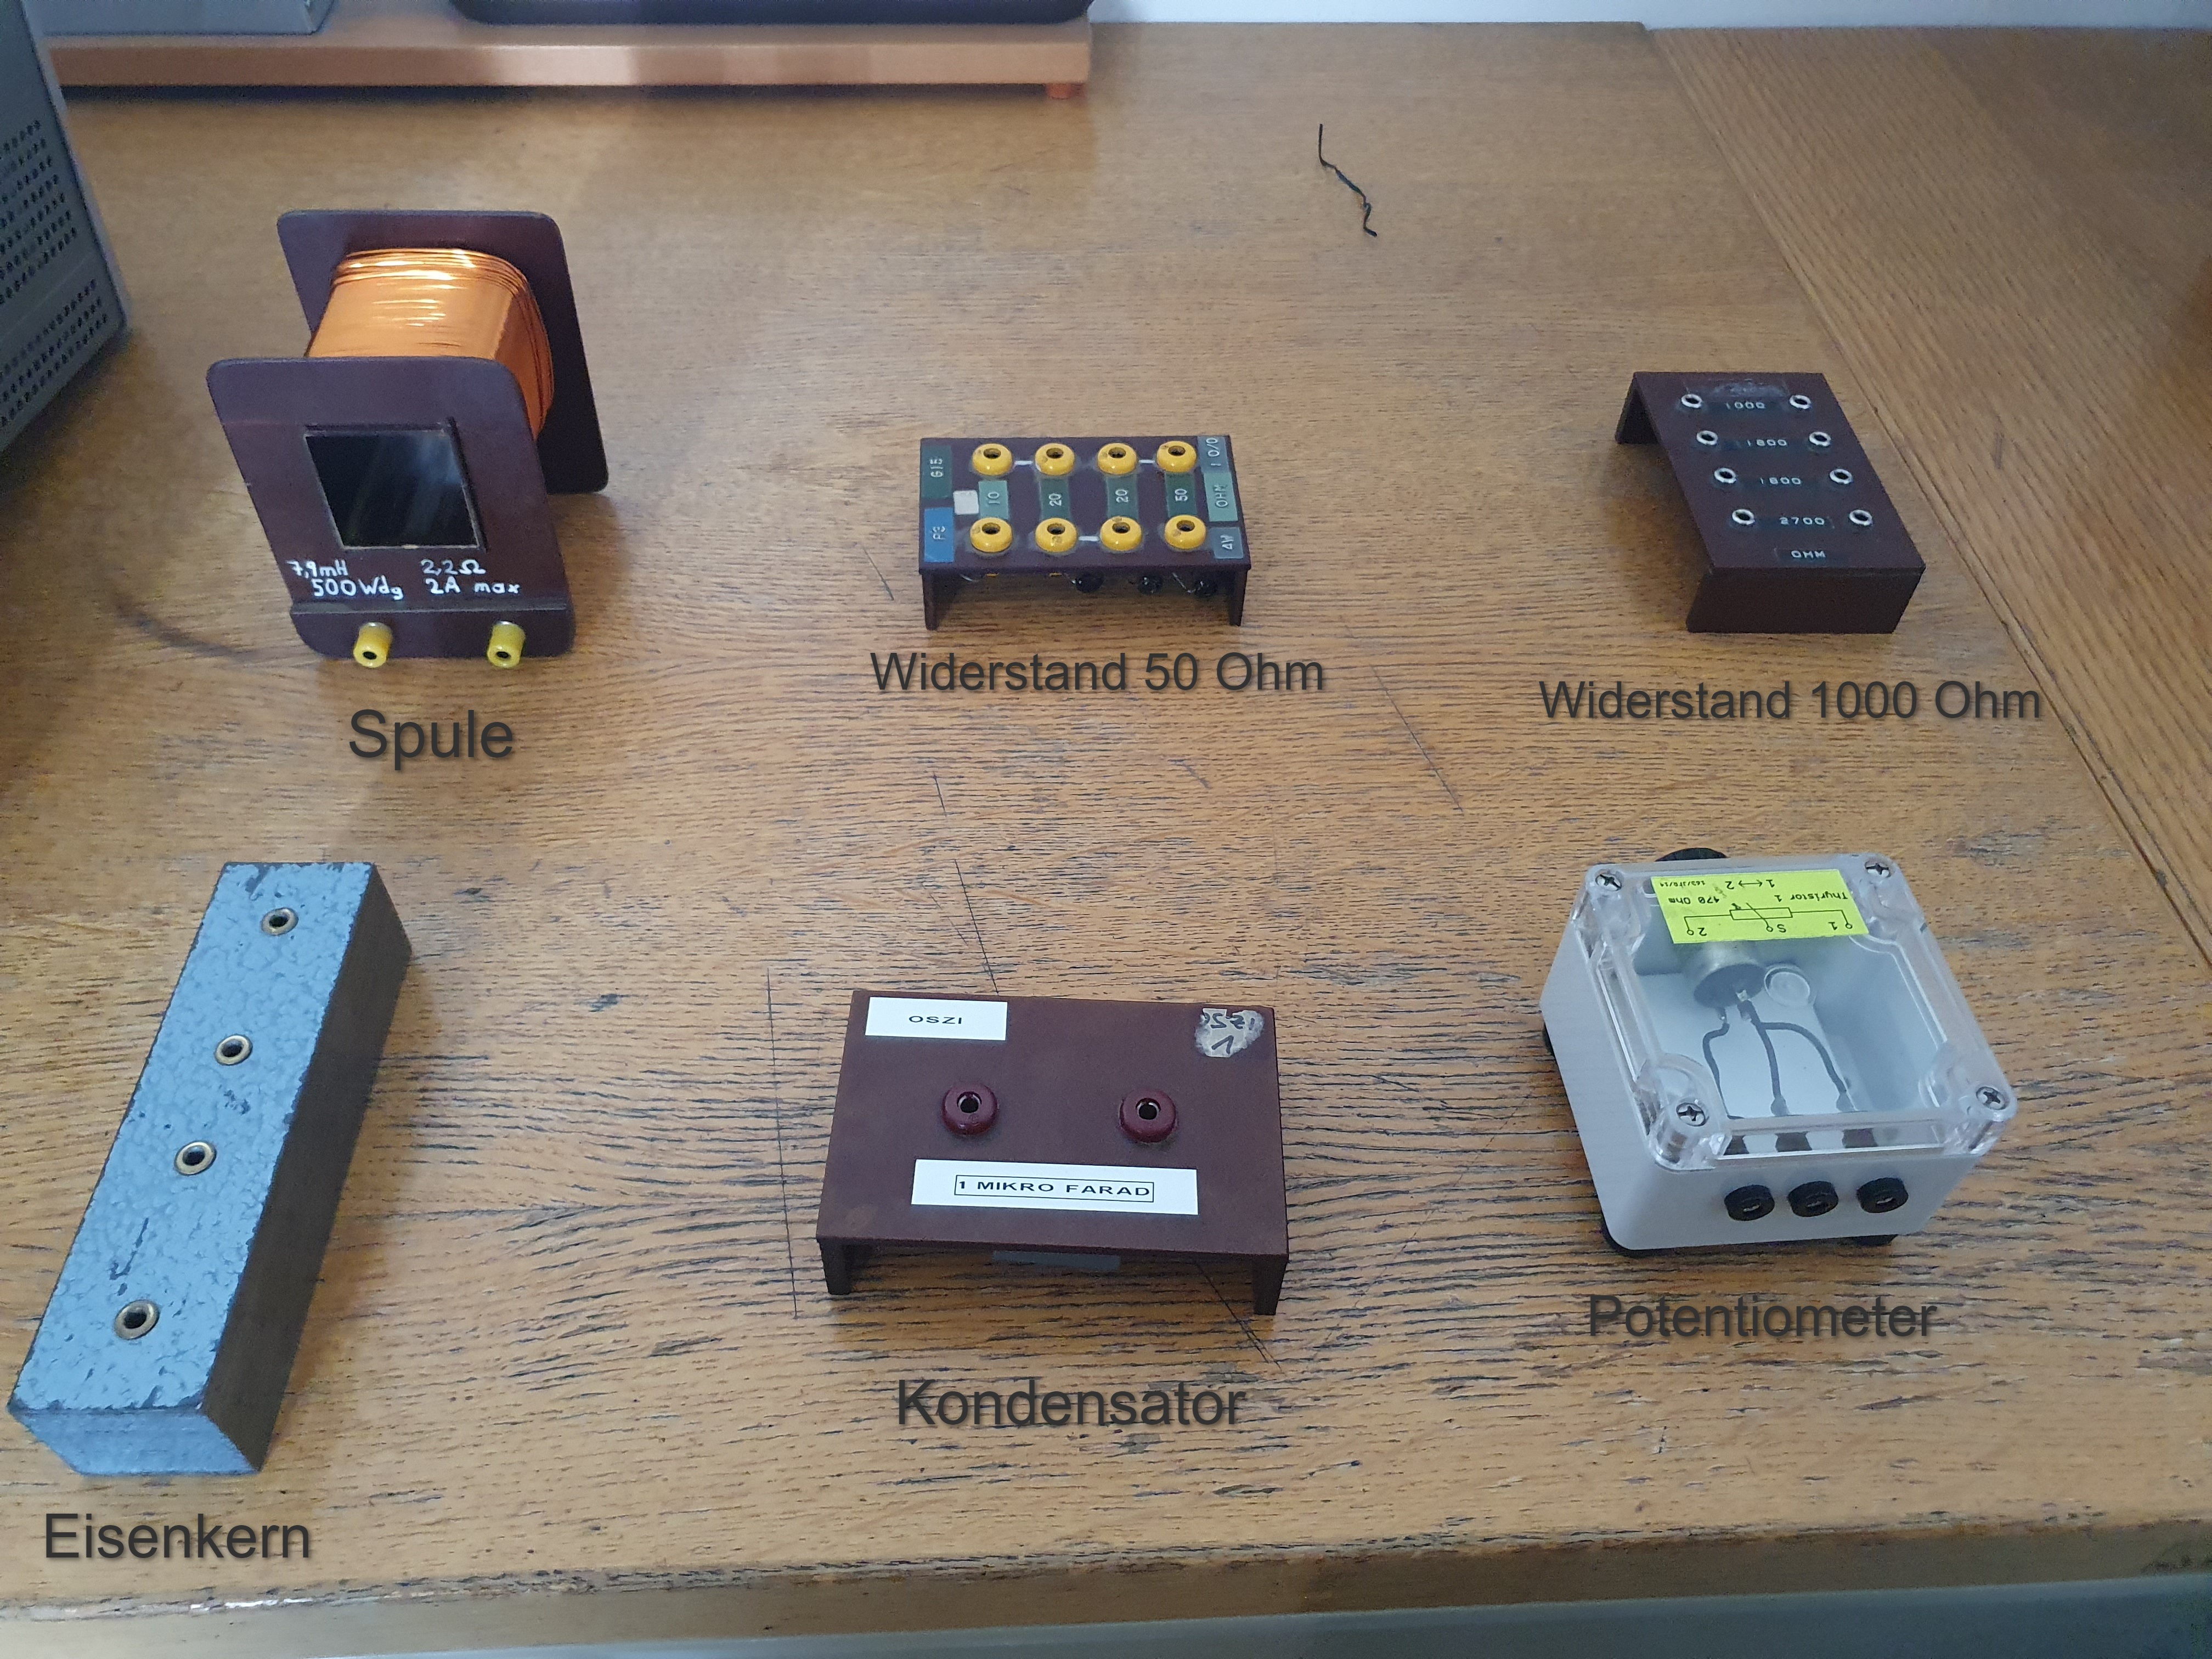
\includegraphics[width=0.6\linewidth, angle=0]{nudes/Utensilien.jpg}
    \caption{Utensilien}
    \label{fig:Utensilien}
\end{figure} 

\noindent
Basierend darauf war der Versuch dann in drei Teilversuche gegliedert. Im ersten Abschnitt davon sollte eine Serienschaltung, bestehend aus einem Widerstand R = 1000 Ohm, einem Kondensator C = 1 $\mu F$, einem Trafo und einem Frequenzgenerator aufgebaut- und dann an das Oszilloskop angeschlossen werden.
Der Schaltplan hierzu ist in folgender Abbildung zu erkennen:

\begin{figure}[H]
    \centering
    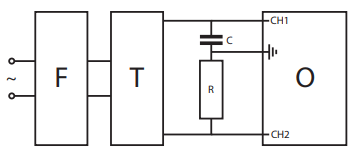
\includegraphics[width=0.6\linewidth, angle=0]{nudes/3.2 Schaltplan.png}
    \caption{Schaltplan Serienschaltung}
    \label{fig:Schaltplan Serienschaltung}
\end{figure}

\noindent
Praktisch aufgebaut sieht der Versuch wie folgt aus:

\begin{figure}[H]
    \centering
    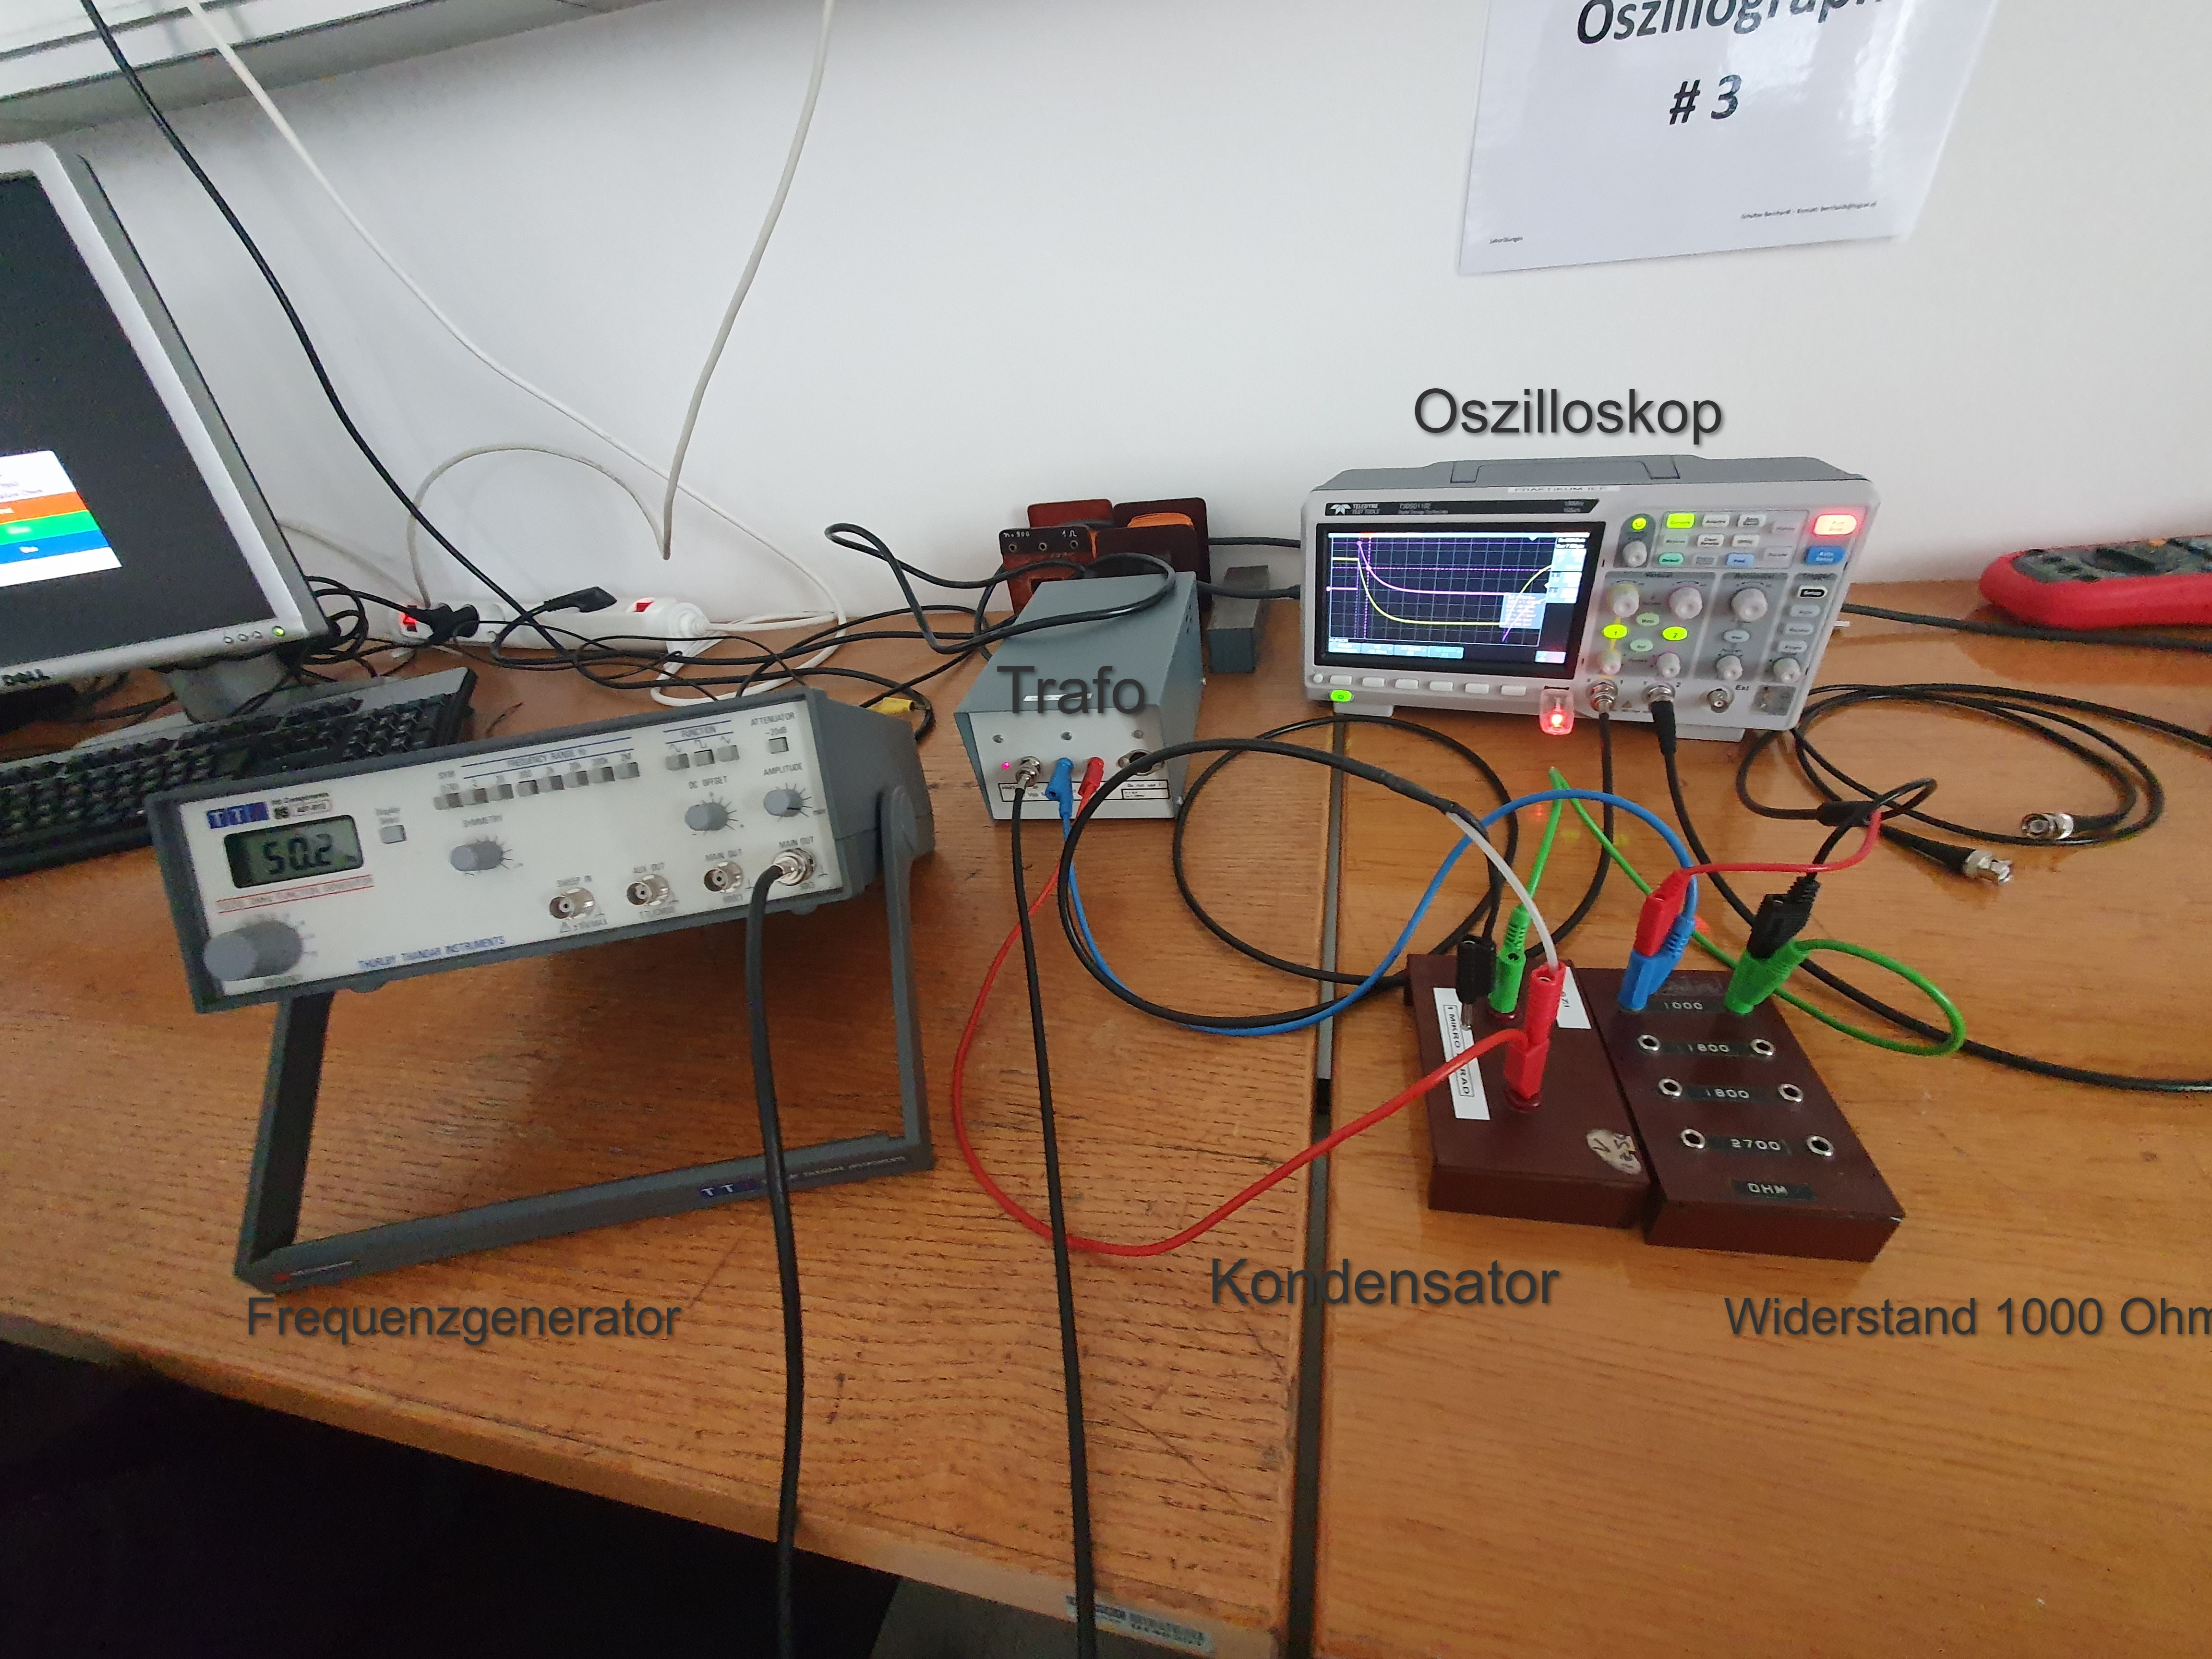
\includegraphics[width=0.6\linewidth, angle=0]{nudes/Aufbau Serienschaltung.jpg}
    \caption{Aufbau Serienschaltung}
    \label{fig:Aufbau Serienschaltung}
\end{figure} 

\noindent
Der Aufbau des zweiten Teiles kann sich mit der Grafik zum Schaltplan des Serienschwingkreises vorgestellt werden:

\begin{figure}[H]
    \centering
    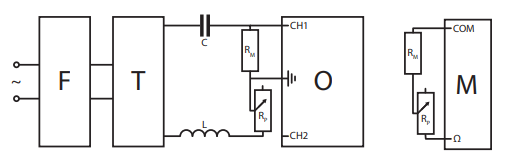
\includegraphics[width=0.6\linewidth, angle=0]{nudes/3.3 Serienschwingkreis.png}
    \caption{Schaltplan Serienschwingkreis}
    \label{fig:Schaltplan Serienschwingkreis}
\end{figure}

\noindent
In der Realität sieht die aufgebaute Schaltung dann so aus:

\begin{figure}[H]
    \centering
    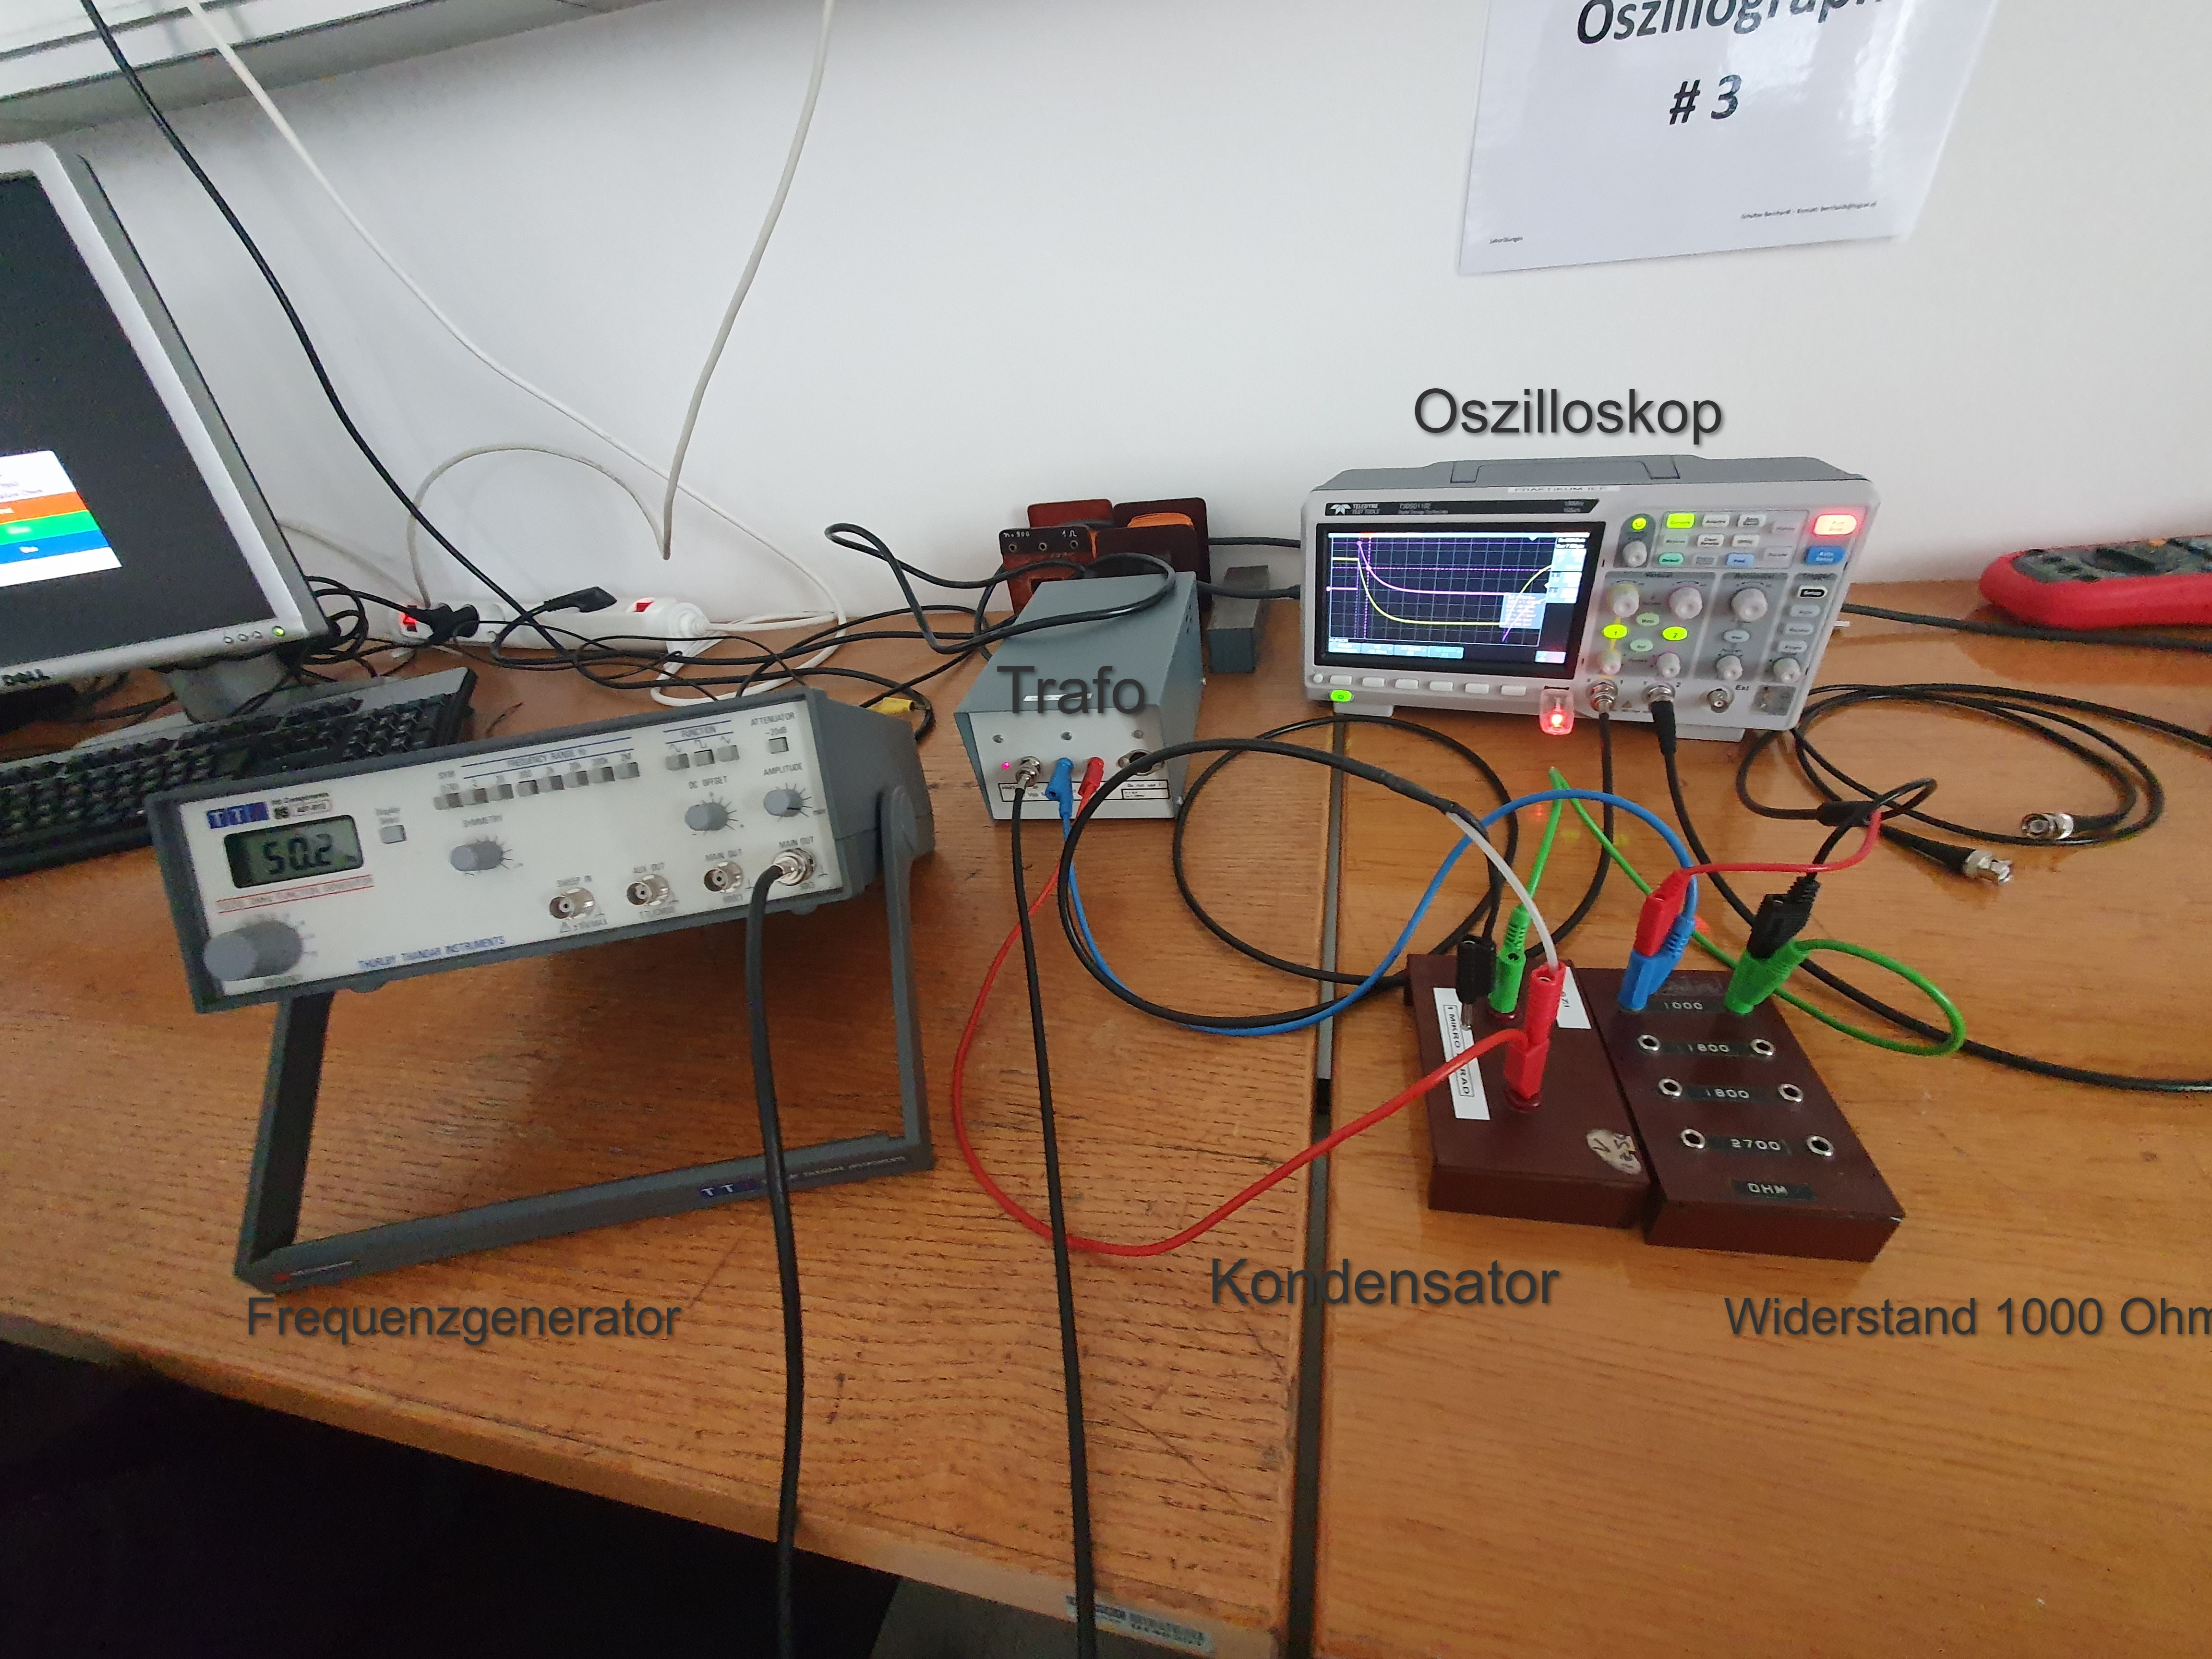
\includegraphics[width=0.6\linewidth, angle=0]{nudes/Aufbau Serienschaltung.jpg}
    \caption{Aufbau Serienschwingkreis}
    \label{fig:Aufbau Serienschwingkreis}
\end{figure} 

\noindent
Die dritte und letzte Schaltung ist im Gegensatz zu den anderen beiden sehr einfach strukturiert und setzt sich lediglich aus zwei Kompnenten zusammen:

\begin{figure}[H]
    \centering
    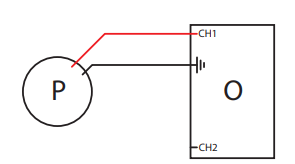
\includegraphics[width=0.6\linewidth, angle=0]{nudes/3.4 Eigenfrequenz.png}
    \caption{Aufbau Serienschaltung}
    \label{fig:Schaltplan Eigenfrequenzbestimmung}
\end{figure}

\noindent
Das Piezo P, welches im dritten Aufgabenteil an das Oszilloskop angeschlossen wird, ist in folgender Abbildung zu sehen:

\begin{figure}[H]
    \centering
    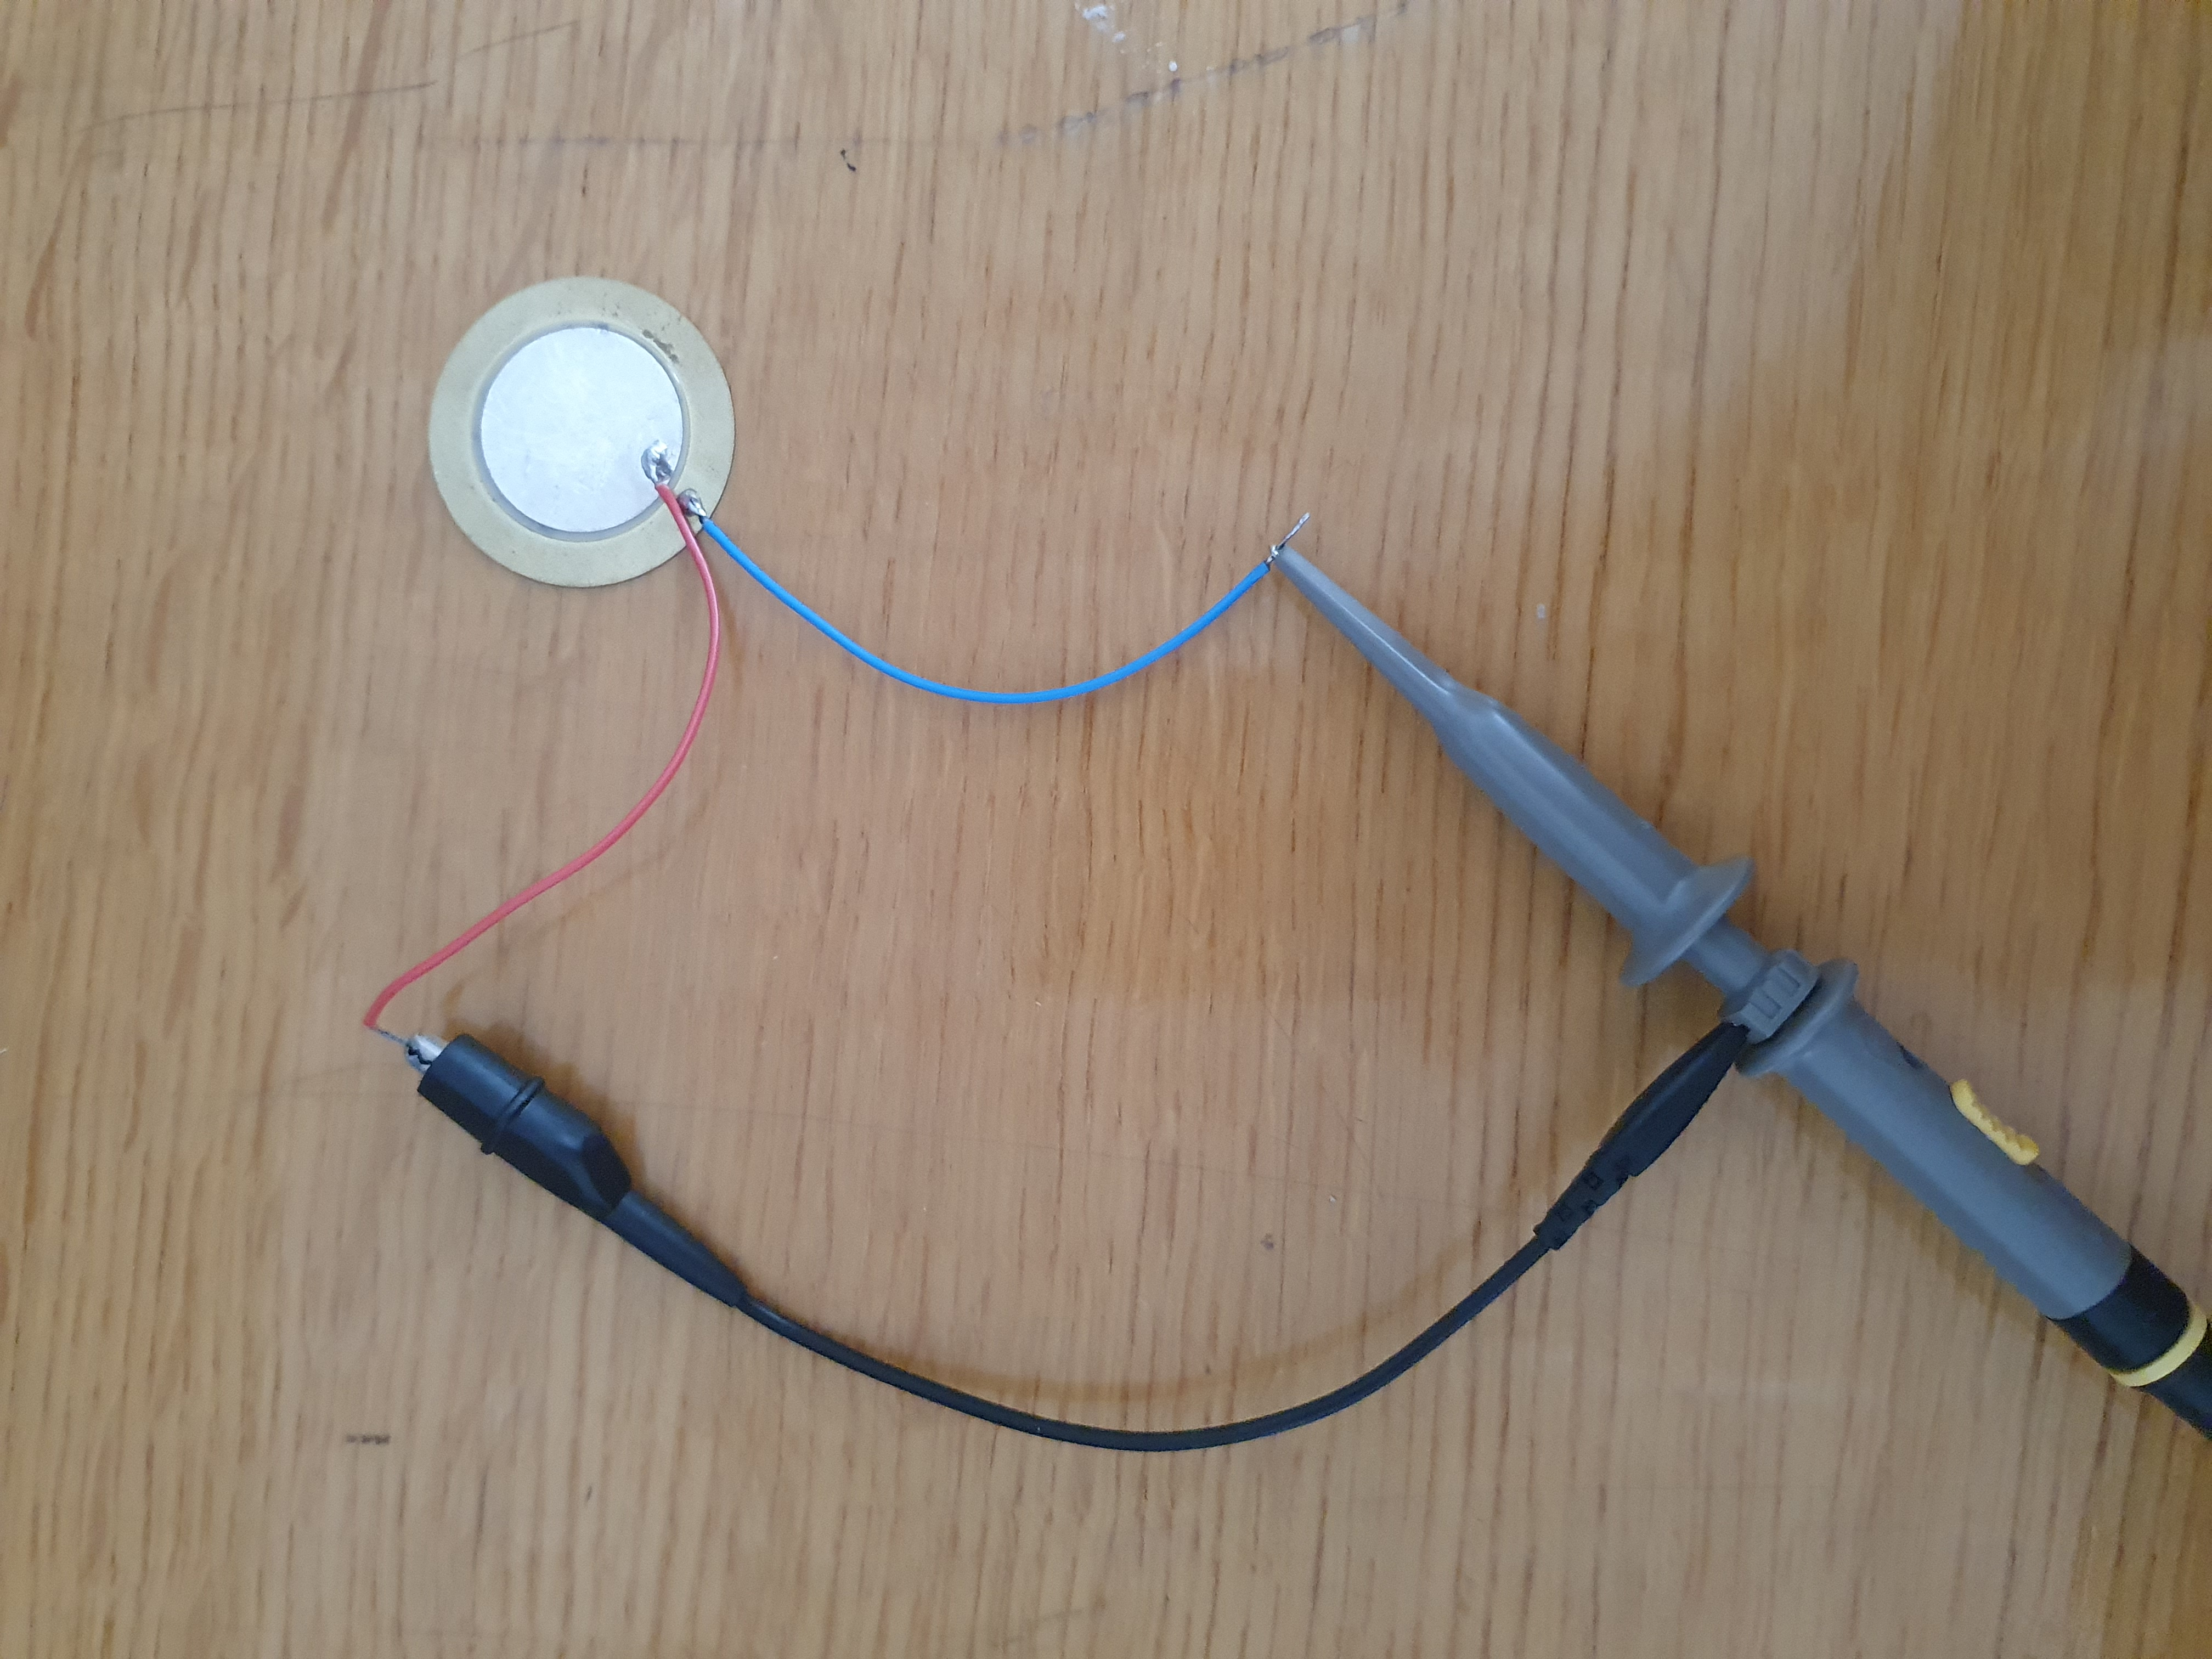
\includegraphics[width=0.6\linewidth, angle=0]{nudes/Piezo.jpg}
    \caption{Piezo}
    \label{fig:Piezo}
\end{figure}



\section{Geräteliste} %jo holt a listn ------------------------------

    \begin{table}[H]
        \centering
        \caption{Im Versuch verwendete Geräte und Utensilien.}
        \label{tab:geraete}
        \begin{tabular}{| l | l | l | l |}
            \hline
            Gerät   & Typ   & Gerätenummer  & Unsicherheit \\
            \hline
            Oszilloskop & {n.a} & {n.a} \\
            Trafo & {n.a} & {n.a} \\
            Frequenzgenerator & {n.a} & {n.a} \\
            Spule mit entfernbaren Eisenkern (n=500) & {n.a} & {n.a} \\
            50 Ohm Widerstand & {n.a} & {n.a} \\
            470 Ohm Potentiometer & {n.a} & {n.a} \\
            50 Ohm / 1000 Ohm Widerstand & {n.a} & {n.a} \\
            1 $\mu F$ Kondensator& {n.a} & {n.a} \\
            Piezo & {n.a} & {n.a} \\
            \hline
        \end{tabular}
    \end{table}


\section{Versuchsdurchführung \& Messergebnisse} %nachvollziehbar und klar dargestellt ------------------------------

Die Unsicherheiten



\section{Auswertung und Unsicherheitsanalyse} %Nicht nur zahlen angeben ------------------------------

In der Auswertung werden zur erhöhten Genauigkeit durchgehend ungerundete Werte bis zu den Endergebnissen verwendet und nur zur Darstellung gerundet. \\
Zur Berechnung der Unsicherheiten wird, wenn nicht anders angegeben, die Größtunsicherheitsmethode verwendet.


\section{Diskussion} %diskussion der Unsicherheiten und Ergebnisse und evtl. verlgeich mit Literatur ------------------------------


\section{Zusammenfassung} %klare, übersichtliche vollständige beantwortung der Aufgabenstellung ------------------------------


\printbibliography[heading=bibintoc]
\end{document}
